% Build:  make -C .. paper-dryrun   (synthetic data, watermarked)   |   make -C .. paper   (real data only)
% JMLR style: place jmlr2e.sty (from jmlr.org/format) next to this file; otherwise an article fallback is used.
\documentclass[11pt]{article}
\IfFileExists{jmlr2e.sty}{\usepackage{jmlr2e}}{\usepackage[margin=1in]{geometry}\newcommand{\editor}[1]{}}
\usepackage[utf8]{inputenc}\usepackage[T1]{fontenc}
\usepackage{amsmath,amssymb,booktabs,graphicx,array,xcolor,fancyhdr,url,hyperref,adjustbox}
\usepackage[numbers,sort&compress]{natbib}
\usepackage{tikz}\usetikzlibrary{shapes.geometric,arrows.meta,positioning,fit}
\tikzset{b/.style={draw,rounded corners=2pt,align=center,font=\scriptsize,minimum width=2.6cm,inner sep=2pt,fill=blue!5},
 d/.style={draw,diamond,aspect=2.2,align=center,font=\scriptsize,inner sep=1pt,fill=yellow!15},
 o/.style={draw,rounded corners=5pt,align=center,font=\scriptsize,inner sep=2pt,fill=green!10},
 ar/.style={-{Stealth[length=4pt]}},lb/.style={font=\tiny,midway}}

\newcommand{\tabdir}{_dryrun/tables}
\newcommand{\figdir}{_dryrun/figures}
\newcommand{\datastatus}{DRYRUN}
                       % \tabdir \figdir \datastatus  (written by build.py)
\newcommand{\dryrunTag}{DRYRUN}
\newcommand{\safeinput}[1]{\IfFileExists{#1.tex}{\input{#1}}{\emph{(not generated: #1)}}}
\newcommand{\rtab}[1]{\begin{adjustbox}{max width=\linewidth}\safeinput{\tabdir/#1}\end{adjustbox}}
\newcommand{\rfig}[2][0.9]{\IfFileExists{\figdir/#2.pdf}{\includegraphics[width=#1\linewidth]{\figdir/#2.pdf}}{\emph{(missing figure #2)}}}
\newcommand{\R}{R^2}\newcommand{\rfar}{R^2_{\mathrm{far}}}\newcommand{\HX}{HypatiaX}
\pagestyle{fancy}\fancyhf{}\fancyfoot[C]{\thepage}
\ifx\datastatus\dryrunTag\fancyhead[C]{\textcolor{red}{\bfseries DRY-RUN BUILD --- SYNTHETIC DATA --- NOT SCIENTIFIC RESULTS}}\fi
\title{Which Hybrid? A Seven-Variant Comparison of LLM-Guided Symbolic Regression\\for Extrapolation-Reliable Discovery}
\author{Anonymous (draft)}
\date{\today}
\begin{document}\maketitle
\ifx\datastatus\dryrunTag\begin{center}\fbox{\parbox{0.9\linewidth}{\color{red}\textbf{Dry-run build.} Every number, table and figure derived from experiments in this PDF comes from a random generator used to test the pipeline. Nothing here is a finding.}}\end{center}\fi
\begin{abstract}
Hybrid methods that combine a large-language-model (LLM) symbolic prior with neural or evolutionary regressors are usually judged on in-distribution fit, which hides catastrophic extrapolation failures. We compare seven hybrid variants and three baselines under a single protocol that reports far-extrapolation $R^2$, win rate with bootstrap confidence intervals, and per-domain extrapolation behaviour, and we audit each variant for the implementation defects that most threaten such comparisons (silent no-op LLM paths, test-set leakage, version drift). \emph{Results are pending the full experiment run; this abstract will be completed from the final tables.}
\end{abstract}
\section{Introduction}
Symbolic regression (SR) searches for closed-form expressions that explain data \citep{koza1992gp,schmidt2009distilling,cranmer2023pysr}, and promises models that extrapolate because their structure matches the generating law \citep{udrescu2020aifeynman}. Recent work injects LLM priors into SR \citep{shojaee2025llmsr,romeraparedes2024funsearch}. Neural networks, in contrast, fit arbitrary in-distribution structure but extrapolate poorly \citep{xu2021extrapolate,balestriero2021extrapolation}. \HX{} combines these ingredients in several different ways; this paper asks \emph{which} combination is most reliable.
We address three goals: \textbf{G1} the win rate of each hybrid variant against baselines; \textbf{G2} which variant extrapolates best in which domain; \textbf{G3} the advantages and limitations of each variant, including implementation defects found during audit.
Contributions: (i) a frozen taxonomy of seven variants with executable decision flows (Section~\ref{sec:variants}); (ii) a same-cases evaluation protocol with a win-rate definition robust to ties and failed runs (Section~\ref{sec:protocol}); (iii) an audit register that treats leakage, dead code paths and version drift as first-class threats to validity (Section~\ref{sec:threats}).
\section{Related work}
\paragraph{Symbolic regression.} Genetic programming \citep{koza1992gp}, sparse regression over libraries \citep{brunton2016sindy}, reinforcement-learned search \citep{petersen2021dsr} and pre-trained sequence models \citep{biggio2021nsr,kamienny2022e2e} define the landscape; benchmarks include Nguyen \citep{uy2011nguyen}, Feynman \citep{udrescu2020aifeynman} and SRBench \citep{lacava2021srbench}. Equation-learning networks were designed explicitly to extrapolate to unseen input domains for systems governed by analytical expressions \citep{sahoo2018eqldiv}. Exact SR is NP-hard \citep{virgolin2022nphard}, which motivates priors.
\paragraph{LLMs for science.} LLM-guided program and equation search \citep{romeraparedes2024funsearch,shojaee2025llmsr} treats the model as a proposal distribution; LLM-SRBench \citep{shojaee2025llmsrbench} was built specifically to limit memorisation of well-known equations, a concern that applies equally to our LLM-prior variants.
\paragraph{Hybrids and ensembles.} Stacking \citep{wolpert1992stacking} and deep ensembles with predictive uncertainty \citep{lakshminarayanan2017deepensembles} motivate precision-weighted blends; calibration is not guaranteed \citep{guo2017calibration}.
\paragraph{Extrapolation and shift.} Extrapolation is a distribution-shift problem \citep{quinonero2009shift}; neural networks need not extrapolate \citep{xu2021extrapolate,balestriero2021extrapolation}. We use a PCA-directed hold-out of the far end of the first principal component \citep{pearson1901pca} in addition to multiplier-based far splits.
\paragraph{Statistics.} We follow \citet{demsar2006statistical} (Friedman \citep{friedman1937use}, Nemenyi, Wilcoxon \citep{wilcoxon1945ranking} with Holm correction \citep{holm1979simple}) and percentile bootstrap intervals \citep{efron1993bootstrap}.
\section{The seven variants}\label{sec:variants}
Table~\ref{tab:variants} fixes the identifiers used throughout (resolving a mismatch between source documents, audit A-001). All variants consume an LLM-derived prior; they differ in \emph{where} it enters.
\begin{table}[t]\centering\small\rtab{t1_variants}\caption{Variants and baselines. Registry = index passed to the runner.}\label{tab:variants}\end{table}
\begin{description}\setlength\itemsep{0pt}
\item[V1] LLM formula $\to$ scipy constant refit (accepted if train $\R$ improves by $>0.001$) $\to$ gate: \emph{fitted-symbolic} if $\R_{fit}\ge0.85$ and margin $>0.05$; \emph{ensemble} if both $\ge0.5$ and $|\text{margin}|\le0.15$; else NN.
\item[V2] Tie-favours-symbolic gate ($\R_{llm}\ge\R_{nn}$), \texttt{force\_llm} override for known physics families, blend only if NN wins with $\R_{nn}>0.90$.
\item[V3] Precision-weighted blend of LLM and NN predictions, no hard gate. \emph{Weighting differs between our sources (audit A-007) and is fixed by the implementation actually run.}
\item[V4] \texttt{SymbolicEngineWithLLM}: modes \emph{none/seed/hybrid/fallback}; hybrid returns the LLM formula if $\R>0.95$, discards it if $<0.5$, else seeds PySR and keeps the better; fallback runs PySR first and calls the LLM only if $\R\le0.90$.
\item[V5] A retry loop around one search engine (up to five attempts, seeds $42{+}k$, early stop at $\R\ge0.95$) with an optional physics-aware regressor, \emph{disabled by default} (A-006). It consumes up to five times V4's search budget (A-022); Table~\ref{tab:cost} reports cost.
\item[V6] Validation-selected residual hybrid (DeFi): candidate pool \{LLM, NN$\times2$, residual-NN, blend over a 21-point grid, linear fallback\}, chosen on an edge validation slice taken from the high end of the \emph{training} range; an extrapolation guard removes bare NN candidates when the test domain leaves the training range.
\item[V7] LLM candidates are converted to PySR \texttt{guesses} \emph{before} search (population seeding), compared with an unseeded run on the same case; the run refuses to start if the engine cannot accept guesses.
\end{description}
\begin{figure}[t]\centering\begin{minipage}[t]{0.33\linewidth}\centering\textbf{V1}\\[2pt]
\resizebox{\linewidth}{!}{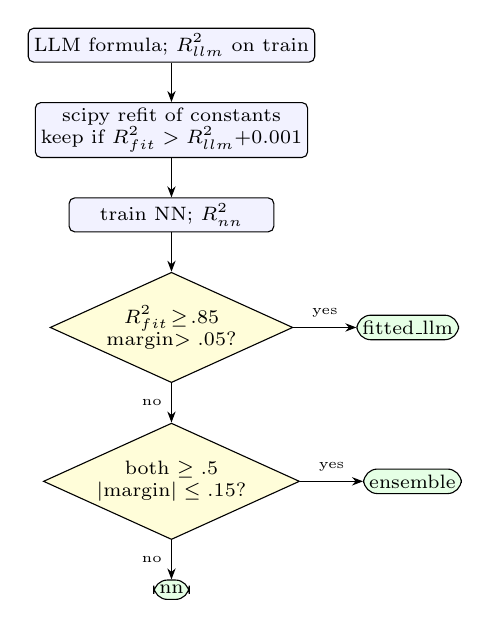
\begin{tikzpicture}[node distance=5mm]
\node[b](a){LLM formula; $\R_{llm}$ on train};\node[b,below=of a](b){scipy refit of constants\\keep if $\R_{fit}>\R_{llm}{+}0.001$};
\node[b,below=of b](c){train NN; $\R_{nn}$};\node[d,below=of c](d){$\R_{fit}\!\ge\!.85$\\margin$>.05$?};
\node[o,right=8mm of d](e){fitted\_llm};\node[d,below=of d](f){both $\ge.5$\\$|$margin$|\le.15$?};
\node[o,right=8mm of f](g){ensemble};\node[o,below=of f](h){nn};
\draw[ar](a)--(b);\draw[ar](b)--(c);\draw[ar](c)--(d);\draw[ar](d)--node[lb,above]{yes}(e);\draw[ar](d)--node[lb,left]{no}(f);
\draw[ar](f)--node[lb,above]{yes}(g);\draw[ar](f)--node[lb,left]{no}(h);\end{tikzpicture}}\end{minipage}%
\begin{minipage}[t]{0.33\linewidth}\centering\textbf{V2}\\[2pt]
\resizebox{\linewidth}{!}{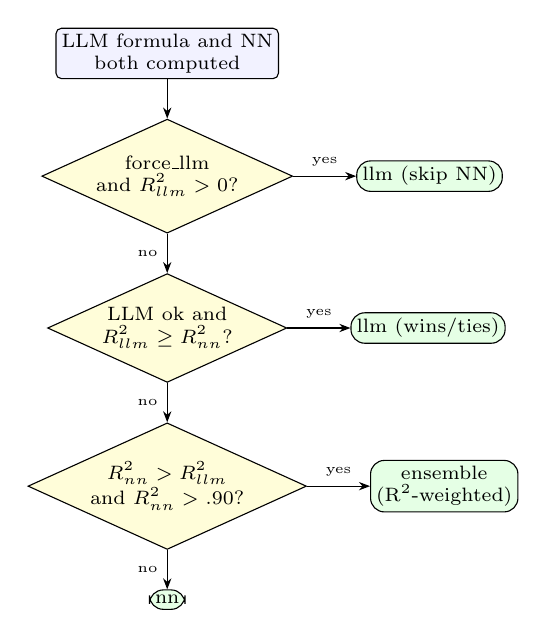
\begin{tikzpicture}[node distance=5mm]
\node[b](a){LLM formula and NN\\both computed};\node[d,below=of a](b){force\_llm\\and $\R_{llm}>0$?};
\node[o,right=8mm of b](c){llm (skip NN)};\node[d,below=of b](d){LLM ok and\\$\R_{llm}\ge\R_{nn}$?};
\node[o,right=8mm of d](e){llm (wins/ties)};\node[d,below=of d](f){$\R_{nn}>\R_{llm}$\\and $\R_{nn}>.90$?};
\node[o,right=8mm of f](g){ensemble\\(R$^2$-weighted)};\node[o,below=of f](h){nn};
\draw[ar](a)--(b);\draw[ar](b)--node[lb,above]{yes}(c);\draw[ar](b)--node[lb,left]{no}(d);\draw[ar](d)--node[lb,above]{yes}(e);
\draw[ar](d)--node[lb,left]{no}(f);\draw[ar](f)--node[lb,above]{yes}(g);\draw[ar](f)--node[lb,left]{no}(h);\end{tikzpicture}}\end{minipage}%
\begin{minipage}[t]{0.33\linewidth}\centering\textbf{V3}\\[2pt]
\resizebox{\linewidth}{!}{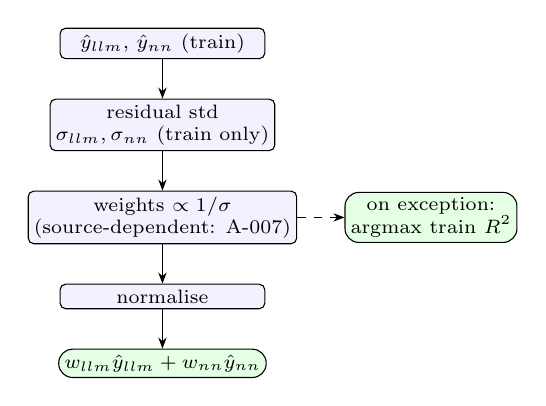
\begin{tikzpicture}[node distance=5mm]
\node[b](a){$\hat y_{llm}$, $\hat y_{nn}$ (train)};\node[b,below=of a](b){residual std\\$\sigma_{llm},\sigma_{nn}$ (train only)};
\node[b,below=of b](c){weights $\propto 1/\sigma$\\(source-dependent: A-007)};\node[b,below=of c](d){normalise};
\node[o,below=of d](e){$w_{llm}\hat y_{llm}+w_{nn}\hat y_{nn}$};\node[o,right=6mm of c](f){on exception:\\argmax train $\R$};
\draw[ar](a)--(b);\draw[ar](b)--(c);\draw[ar](c)--(d);\draw[ar](d)--(e);\draw[ar,dashed](c)--(f);\end{tikzpicture}}\end{minipage}
\caption{Decision flows of V1--V3.}\label{fig:flow1}\end{figure}
\begin{figure}[t]\centering\begin{minipage}[t]{\linewidth}\centering\textbf{V4 (llm\_mode)}\\[2pt]
\resizebox{\linewidth}{!}{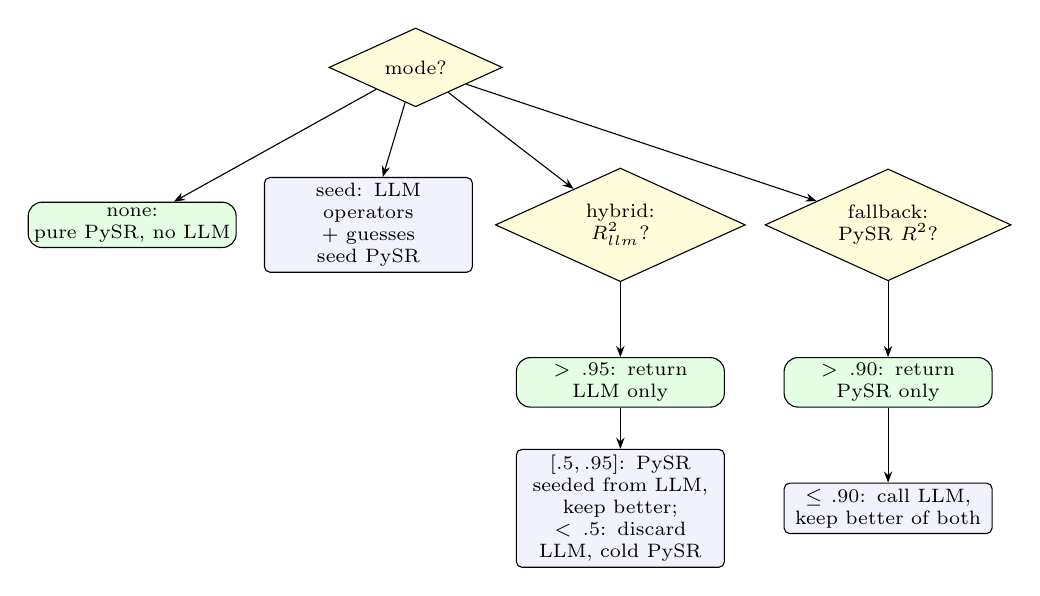
\begin{tikzpicture}[every node/.append style={text width=2.5cm}]
\node[d,text width=1.6cm](m) at (3.6,0){mode?};
\node[o](n) at (0,-2){none:\\pure PySR, no LLM};
\node[b](s) at (3.0,-2){seed: LLM operators\\+ guesses seed PySR};
\node[d,text width=1.8cm](h) at (6.2,-2){hybrid:\\$\R_{llm}$?};
\node[d,text width=1.8cm](f) at (9.6,-2){fallback:\\PySR $\R$?};
\node[o](h1) at (6.2,-4){$>.95$: return LLM only};
\node[b](h2) at (6.2,-5.6){$[.5,.95]$: PySR seeded from LLM, keep better;\\$<.5$: discard LLM, cold PySR};
\node[o](f1) at (9.6,-4){$>.90$: return PySR only};
\node[b](f2) at (9.6,-5.6){$\le.90$: call LLM,\\keep better of both};
\draw[ar](m)--(n);\draw[ar](m)--(s);\draw[ar](m)--(h);\draw[ar](m)--(f);
\draw[ar](h)--(h1);\draw[ar](h1)--(h2);\draw[ar](f)--(f1);\draw[ar](f1)--(f2);
\end{tikzpicture}}\end{minipage}\\[6mm]
\begin{minipage}[t]{0.5\linewidth}\centering\textbf{V5 (retry + fallback)}\\[2pt]
\resizebox{\linewidth}{!}{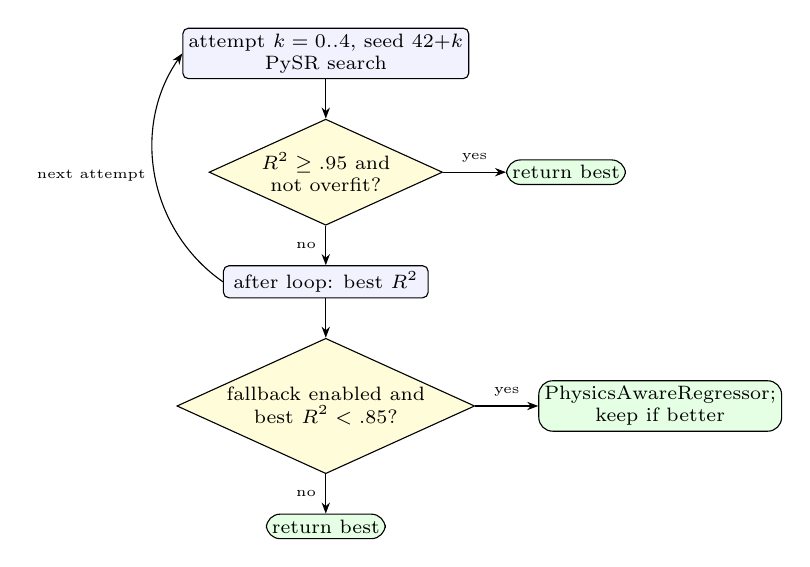
\begin{tikzpicture}[node distance=5mm]
\node[b](a){attempt $k=0..4$, seed $42{+}k$\\PySR search};\node[d,below=of a](b){$\R\ge.95$ and\\not overfit?};
\node[o,right=8mm of b](c){return best};\node[b,below=of b](d){after loop: best $\R$};
\node[d,below=of d](e){fallback enabled and\\best $\R<.85$?};\node[o,right=8mm of e](f){PhysicsAwareRegressor;\\keep if better};\node[o,below=of e](g){return best};
\draw[ar](a)--(b);\draw[ar](b)--node[lb,above]{yes}(c);\draw[ar](b)--node[lb,left]{no}(d);\draw[ar,bend left=45](d.west)to node[lb,left]{next attempt}(a.west);
\draw[ar](d)--(e);\draw[ar](e)--node[lb,above]{yes}(f);\draw[ar](e)--node[lb,left]{no}(g);\end{tikzpicture}}\end{minipage}%
\begin{minipage}[t]{0.5\linewidth}\centering\textbf{V6 (validation-selected, DeFi)}\\[2pt]
\resizebox{\linewidth}{!}{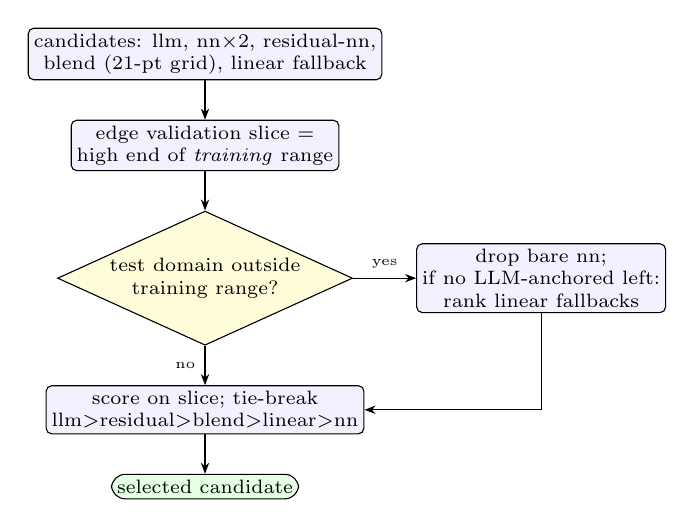
\begin{tikzpicture}[node distance=5mm]
\node[b](a){candidates: llm, nn$\times2$, residual-nn,\\blend (21-pt grid), linear fallback};
\node[b,below=of a](b){edge validation slice =\\high end of \emph{training} range};
\node[d,below=of b](c){test domain outside\\training range?};\node[b,right=8mm of c](d){drop bare nn;\\if no LLM-anchored left:\\rank linear fallbacks};
\node[b,below=of c](e){score on slice; tie-break\\llm$>$residual$>$blend$>$linear$>$nn};\node[o,below=of e](f){selected candidate};
\draw[ar](a)--(b);\draw[ar](b)--(c);\draw[ar](c)--node[lb,above]{yes}(d);\draw[ar](c)--node[lb,left]{no}(e);\draw[ar](d)|-(e);\draw[ar](e)--(f);\end{tikzpicture}}\end{minipage}\\[6mm]
\begin{minipage}[t]{0.5\linewidth}\centering\textbf{V7 (PySR population seeding)}\\[2pt]
\resizebox{\linewidth}{!}{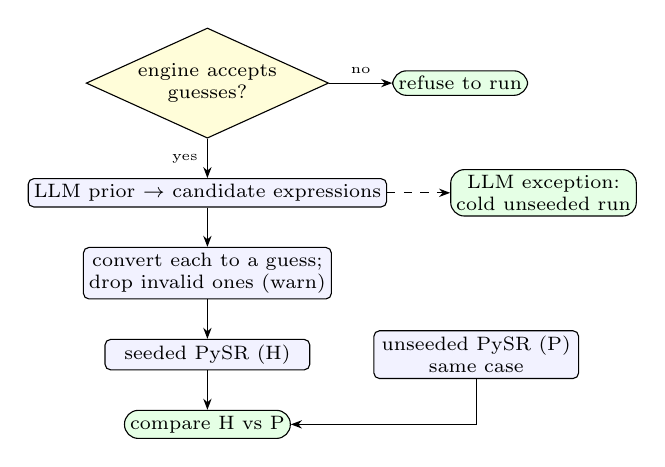
\begin{tikzpicture}[node distance=5mm]
\node[d](a){engine accepts\\guesses?};\node[o,right=8mm of a](x){refuse to run};
\node[b,below=of a](b){LLM prior $\to$ candidate expressions};\node[b,below=of b](c){convert each to a guess;\\drop invalid ones (warn)};
\node[b,below=of c](d){seeded PySR (H)};\node[b,right=8mm of d](e){unseeded PySR (P)\\same case};\node[o,below=of d](f){compare H vs P};
\node[o,right=8mm of b](g){LLM exception:\\cold unseeded run};
\draw[ar](a)--node[lb,above]{no}(x);\draw[ar](a)--node[lb,left]{yes}(b);\draw[ar](b)--(c);\draw[ar](c)--(d);\draw[ar](d)--(f);\draw[ar](e)|-(f);\draw[ar,dashed](b)--(g);\end{tikzpicture}}\end{minipage}
\caption{Decision flows of V4--V7.}\label{fig:flow2}\end{figure}
\begin{figure}[t]\centering\resizebox{\linewidth}{!}{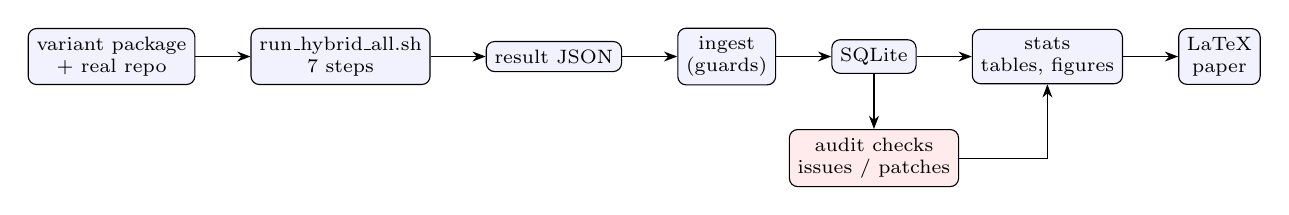
\begin{tikzpicture}[node distance=7mm,every node/.style={draw,rounded corners=3pt,align=center,font=\scriptsize,fill=blue!5,inner sep=3pt}]
\node(a){variant package\\+ real repo};\node[right=of a](b){run\_hybrid\_all.sh\\7 steps};\node[right=of b](c){result JSON};
\node[right=of c](d){ingest\\(guards)};\node[right=of d](e){SQLite};\node[right=of e](f){stats\\tables, figures};\node[right=of f](g){LaTeX\\paper};
\node[below=of e,fill=red!8](h){audit checks\\issues / patches};
\foreach\x/\y in {a/b,b/c,c/d,d/e,e/f,f/g}{\draw[-{Stealth}](\x)--(\y);}
\draw[-{Stealth}](e)--(h);\draw[-{Stealth}](h)-|(f);\end{tikzpicture}}
\caption{Study pipeline: package $\to$ experiments $\to$ database $\to$ paper.}\label{fig:pipeline}\end{figure}
\section{Experimental protocol}\label{sec:protocol}
\paragraph{Experiments.} Seven steps (Table~\ref{tab:exps}) run four protocols (DeFi, Feynman, Nguyen-12, all-30) under random, PCA-directed or far splits. A variant runs only on protocols it declares support for; comparisons never pool across protocols and never rank a method on cases it did not run (same-cases rule). Variant V7 runs only on Nguyen-12.
\begin{table}[t]\centering\small\rtab{t3_experiments}\caption{Experiment inventory (mirrors \texttt{run\_hybrid\_all.sh}).}\label{tab:exps}\end{table}
\paragraph{Metrics.} Primary: far-extrapolation $\rfar$ on the five-tier ladder; secondary: in-distribution test $\R$, near-perfect rate ($\rfar>0.99$), catastrophic rate ($\rfar<-1$), RMSE, MAE.
\paragraph{Win rate.} Per case, the score of a method is the median over seeds of $\rfar$ (failed runs score $-\infty$). The method with the highest score wins; all methods within $0.01$ of the best share a tie and receive $0.5$ each (so tied win scores can sum above one). The win rate is the mean over cases with a 10\,000-resample percentile bootstrap interval (resampling cases). We also report pairwise win matrices, Friedman with Nemenyi critical difference, and Wilcoxon--Holm tests.
\paragraph{Hyper-parameters.} Table~\ref{tab:hp}.
\begin{table}[t]\centering\small\rtab{t14_hparams}\caption{Hyper-parameters and thresholds.}\label{tab:hp}\end{table}

\section{Results}\label{sec:results}
\ifx\datastatus\dryrunTag{\color{red}\emph{All entries in this section come from a synthetic generator and exist only to exercise the pipeline.}}\fi
\subsection{Win rate (G1)}
Table~\ref{tab:wr1} gives win rates on the DeFi random split and Table~\ref{tab:wr2} on Feynman; Figure~\ref{fig:wr} shows all experiments. Pairwise matrices and rank statistics are in Appendix~\ref{app:b}. Nguyen-12 steps run V7 only, so no win rate is defined there (audit A-005).
\begin{table}[t]\centering\scriptsize\rtab{t4_winrate_exp1}\caption{Win rate, DeFi random split.}\label{tab:wr1}\end{table}
\begin{table}[t]\centering\scriptsize\rtab{t4_winrate_exp2}\caption{Win rate, Feynman.}\label{tab:wr2}\end{table}
\begin{figure}[t]\centering\rfig[1.0]{f3_winrate}\caption{Win rate with 95\% bootstrap CI, per experiment.}\label{fig:wr}\end{figure}
Friedman/Nemenyi (DeFi): \safeinput{\tabdir/friedman_exp1}.\quad (Feynman): \safeinput{\tabdir/friedman_exp2}.
\begin{table}[t]\centering\scriptsize\rtab{t7_rates_exp1}\caption{Near-perfect and catastrophic rates, DeFi.}\label{tab:rates}\end{table}
\begin{table}[t]\centering\scriptsize\rtab{t8_decisions}\caption{Gate decision shares.}\label{tab:gate}\end{table}
\subsection{Extrapolation by domain (G2)}
\begin{table}[t]\centering\scriptsize\rtab{t6_domain_exp1}\caption{Median [IQR] of $\rfar$ by domain, DeFi random split.}\label{tab:dom1}\end{table}
\begin{table}[t]\centering\scriptsize\rtab{t6_domain_exp1_pca}\caption{Same, PCA-directed split.}\label{tab:dom2}\end{table}
\begin{table}[t]\centering\scriptsize\rtab{t6_domain_exp2}\caption{Same, Feynman domains.}\label{tab:dom3}\end{table}
\begin{figure}[t]\centering\rfig[0.8]{f4_heatmap_exp1}\rfig[0.8]{f4_heatmap_exp2}\caption{Median far $\R$ by domain and variant (colour clipped to $[-1,1]$).}\label{fig:heat}\end{figure}
\begin{figure}[t]\centering\rfig[0.6]{f10_random_vs_pca}\caption{Paired change in far $\R$ from random to PCA-directed split.}\label{fig:pca}\end{figure}
\subsection{Ablations, noise and sample size}
Seeded vs.\ unseeded (Table~\ref{tab:seed}) and noise/sample-complexity sweeps (Table~\ref{tab:noise}) are ingested through a normalised CSV contract (\texttt{scripts/ingest\_sweeps.py}); adapters from the original scripts' output are validated separately (audit A-010, A-011).
\begin{table}[t]\centering\small\safeinput{\tabdir/t9_seeded}\caption{Seeded vs.\ unseeded.}\label{tab:seed}\end{table}
\begin{table}[t]\centering\small\safeinput{\tabdir/t10_noise_sample}\caption{Noise and sample-size sensitivity.}\label{tab:noise}\end{table}
\begin{figure}[t]\centering\rfig[0.48]{f7_noise}\rfig[0.48]{f8_sample_complexity}\caption{Far $\R$ versus noise level (left) and training-set size (right).}\label{fig:sweeps}\end{figure}
\begin{table}[t]\centering\scriptsize\rtab{t13_cost_exp1}\caption{Compute and API cost per variant (DeFi).}\label{tab:cost}\end{table}
\section{Advantages and limitations (G3)}\label{sec:discussion}
Table~\ref{tab:advlim} summarises the advantages and limitations that follow from the decision logic and from the audit; the empirical columns of Section~\ref{sec:results} qualify them. Three cross-cutting limitations recur. (1) The V1/V2 gates select on \emph{training} $\R$, so nothing in the gate protects against a model that overfits and then extrapolates badly; V6 is the only variant selecting on held-out edge data. (2) Ensemble weighting is defined three different ways across V1--V3, so ``ensemble'' is not one component. (3) Several variants execute LLM-generated code with \texttt{exec}, with only a restricted namespace as isolation.
\begin{table}[t]\centering\scriptsize\rtab{t11_adv_lim}\caption{Advantages and limitations per variant.}\label{tab:advlim}\end{table}
\paragraph{Reliability discrepancy.} One DeFi case (Portfolio Variance) reports $\R=1.000$ in-sample and $\rfar=-882.9$ at seed 42 for the same variant. Figure~\ref{fig:trainfar} shows train versus far $\R$ over all runs; the experiment \texttt{hybrid\_exp1b} is its multi-seed sweep. We do not average this case away.
\begin{figure}[t]\centering\rfig[0.55]{f6_train_vs_far}\caption{Train vs.\ far $\R$ (symlog axis).}\label{fig:trainfar}\end{figure}
\section{Threats to validity and audit}\label{sec:threats}
\paragraph{Leakage.} Two classes were recorded in the source history: prompts that embedded the expected formula, and ensemble weights computed from test residuals \citep{zhang2017rethinking}. We scan prompt-building code for ground-truth tokens and residual-std expressions (Appendix~\ref{app:a}); static hits are leads for manual review, not verdicts.
\paragraph{Dead LLM path.} Before engine v5.0 the \texttt{use\_llm} flag was a silent no-op, so ``hybrid'' V4/V5 results from older builds are pure PySR. Every stored run carries its engine version and rows below 5.0 are rejected at ingestion; rows without a version are flagged.
\paragraph{Compute confound.} V5 may use up to five search attempts per case; win rates between V5 and single-run variants are therefore not budget-matched (Table~\ref{tab:cost}).
\paragraph{Non-determinism.} LLM output at temperature 0 is not guaranteed byte-identical across requests; a freeze cache removes variance only for repeated prompts. Seeds, engine version, git SHA and API-call counts are stored per run.
\paragraph{Audit register.} Table~\ref{tab:audit} lists issues, patches and the fix rate.
\begin{table}[t]\centering\scriptsize\rtab{t12_audit}\caption{Audit register.}\label{tab:audit}\end{table}
\section{Conclusion}
\emph{To be written from the final results.} The study answers G1--G3 only after the experiments in Table~\ref{tab:exps} are run on the real repository; the contributions that stand independently are the frozen taxonomy, the same-cases win-rate protocol and the audit register.

\bibliographystyle{plainnat}\bibliography{references}
\appendix\section{Reproducibility}\label{app:a}
Repository layout, commands and the audit procedure are in \texttt{GUIDE\_FOR\_IMPLEMENTATION.md} and \texttt{AGENT\_PLAYBOOK.md}. Experiments run through \texttt{scripts/run\_hybrid\_all.sh}; results are ingested with \texttt{scripts/ingest\_results.py} and all tables and figures are rebuilt by \texttt{rsc/experiments/analytics/build.py}.
\begin{table}[h]\centering\small\rtab{t2_coverage}\caption{Variant $\times$ experiment coverage (number of cases).}\end{table}
\section{Per-experiment statistics}\label{app:b}
\begin{table}[h]\centering\tiny\rtab{t5_pairwise_exp1}\caption{Pairwise win rate, DeFi random (row beats column).}\end{table}
\begin{table}[h]\centering\small\rtab{t5b_ranks_exp1}\caption{Average Friedman ranks, DeFi random.}\end{table}

\end{document}
